% Chapter 1

\chapter{Introduction} % Write in your own chapter title
\label{Chapter:Intro}
\lhead{Chapter 1. \emph{Introduction}} % Write in your own chapter title to set the page header
\begin{center}
\textit{
Say first, of God above, or man below,\newline
What can we reason, but from what we know?\newline
Of man what see we, but his station here,\newline
From which to reason, or to which refer?\newline
Through worlds unnumber'd though the God be known,\newline
'Tis ours to trace him only in our own.\newline
He, who through vast immensity can pierce,\newline
See worlds on worlds compose one universe,\newline
Observe how system into system runs,\newline
What other planets circle other suns,\newline
What varied being peoples ev'ry star,\newline
May tell why Heav'n has made us as we are.\newline
But of this frame the bearings, and the ties,\newline
The strong connections, nice dependencies,\newline
Gradations just, has thy pervading soul\newline
Look'd through? or can a part contain the whole?\newline
\newline
Is the great chain, that draws all to agree,\newline
And drawn supports, upheld by God, or thee?}\newline
- Alexander Pope 1733, `An Essay on Man: Epistle I'
\end{center}

\section{Motivation}
\label{sec:Motivation}

\subsection{The answer we seek.}
%Why did people first start looking at galaxies
The firmament has been the muse of humans for as long as we have recorded our history and most likely longer still. The field of astronomy is descended from priests who worshipped celestial objects as the divine and sought for them to bring meaning to their world. Structures such as Stonehenge use celestial objects to allow people to track the `repetitious' passage of time, thus being able to predict the seasons. It is possible that this correlation between the heavens and the earthly systems so critical to life is the reason that humanity became convinced that the universe was there for our benefit. Elaborate orrerys with the earth at the centre of all creation were built to explain how the sun and planets orbit around us cementing our belief that we are at its origin. 
The progression to modern astronomy was slow. However, thanks to advances in scientific thinking and technological process we have shed many of the biases and limitations that once held us back. We are now able to discover our place in cosmos that is unfathomably enormous, diverse and inhospitable. 

The Milky Way is our home and was the first observed galaxy. The name comes from Greek to mean `milky circle' stemming from our belief that the universe exists to give us life and gives the galaxy a mammalian nurturing characteristic. The idea of complexity emerging from the universe is present in the first classification of the structures of galaxies by Edwin Hubble \citep{Hubble1926Extra-galacticNebulae.,Hubble1927TheNebulae}.
Complex spirals were thought to be the descendants of elliptical galaxies leading to the misnomer of `early-type' (elliptical) and `late-type' (spiral) galaxies, as it has since been found that, amongst other formation pathways, it is spiral galaxies that transform into elliptical galaxies. The Universe is at its core in antithesis to the way humanity regards themselves, it thus presents a challenge in thinking to detach hubris and think logically about a system that in its entirety is truly incomprehensible. This must be reflected in galactic modelling we must understand the limitations and scope of our work and the scope of what each model can explain.

Most advances in astronomy have come from technological progress. Beginning from when the most advanced way to view the cosmos was with the naked eye we observed little and interpretations were thus limited. With the advent of optics, such as lenses and then mirrors, which led to the building of telescopes, the ability to look deeper into space became a possibility and the first work on the classification of astrophysical objects was done. Modern advances such as CCD/SED photographic plates, and telescopes that work outside of the visible wavelengths, gave information far beyond what the human eye can see. 

With the influx of new information, galaxy models have become further refined. The emergent complexity proposed by Hubble is superseded by a hierarchical formation which mutates structures. Observations of our galaxy and distant galaxies show how different morphologies of galaxies are more or less common at different masses. Galaxies with different masses and morphologies can be seen to form stars at different rates, with some of the most massive appearing `red and dead'. We also find an `arrow of time' where galaxies seem to increase in star formation peak and drop showing we are likely past the point of maximum stellar mass creation in the Universe. Whilst these discoveries are far more complex then that of those made by studying the sky only with their eye, we are connected by the ultimate pervasive question of `why?'\footnote{42}.

%How has the study of galaxies progressed
\subsection{The tools we use.}
The field of astronomy is both privileged and restricted by observation. No experiment can generate new data and thus it flips the traditional theory, experiment, data, analysis, theory, ... cycle that exists in most other fields. Theoretical, models are often driven by the data and must be careful not to over-fit. Furthermore, for astronomers who observe galactic scale objects, the timescales involved eclipse not only a human lifespan but the entirety of human civilization. It is then fortunate that the finite the speed of light and the distances between galaxies result in observations of the most distant galaxies are also observations of the history of galaxies. By looking at galaxies at different epochs we can construct a picture of how the galactic population has changed and evolved. Under the standard axiom that the Universe is at large scales homogeneous and isotropic, we can assume that the galaxies observed in the far distance, in both time and space, are similar to the progenitors of observed local galaxies that are closer in time and space. Wit knowledge of the start point and endpoint of galaxy populations theories of how galaxies evolve can be given real constraints. To test these theories the ability to model galaxies and `fast forward' time is required such that simulations can provide results in a reasonable time frame.

The first such model by \citet{Holmberg1941OnProcedure.} predates digital computing and used an array of light bulbs where the `candle power', or flux, was a proxy for mass. Two arrays of bulbs were constructed and by measuring the intensity of light along two axes the total gravitational attraction is calculated. The light is a reasonable proxy for mass due to the similarity in the inverse square laws that govern both the spread of light and an increase in the gravitational potential. Each mass element (light bulb) is then given an acceleration and its position updated manually. In the \citet{Holmberg1941OnProcedure.} the merging of two systems of distributed mass is confirmed along with an investigation of the change of shape of the systems. 

With the rapid increase in computing power over the last century, the capability of galaxy simulations has grown. The simulation of mass and mergers have improved with more and smaller `mass elements'. Beyond simply testing the dynamics of mass, simulations also have prescriptions for the formation of stars from gas, the feedback of energy from central black holes millions of times the mass of our sun, feedback from supernovae, and more... \citep[e.g.,][]{McAlpine2015TheCatalogues, Pillepich2018FirstGalaxies}. Despite these major advancements made over many decades, a full understanding of the assembly and evolution of galaxies in our Universe is beyond our capability. Other less computationally intensive analytic tools have been used to model from `first principles', in this instance gas collapse, the formation of galaxy populations. Since their original inception where galaxies form from gas via the loss of angular momentum and cooling to form galactic disks \cite{Mo1998TheDiscs}, these so-called ``Semi-Analytic'' Models have branched out to cover tens of different analytic recipes that try to balance different processes to faithfully recreate the diversity in galaxy populations \citep[e.g.,][]{DeLucia2006TheGalaxies, Guo2011FromCosmology}. A recent development in galactic modelling attempts not to recreate the entire Universe from first principles but to use what we observe as a guide providing powerful constraints. These ``Semi-Empirical Models'' are observation driven and ask focused questions to understand if a given hypothesis for formation is adequate to link the observed galactic population over cosmic history \citep{Hopkins2010MERGERSMATTER, Zavala2012, Moster2013, Shankar2014, Moster2018Emerge10}.

%What questions will we answer
\subsection{The questions we answer.}
In this thesis, we describe \steel, the STastical sEmi-Empirical modeL, PJG's contribution to the galactic modelling community. \steel has been designed to be complementary to existing models of and approaches to galaxy formation. \steel uses semi-empirical modelling techniques but its defining characteristic is its statistical nature. Traditional models, described in more detail below, simulate discrete elements of dark matter extract from a cosmological volume. \steel instead creates a simulation of galaxy populations using number density functions to describe cosmological volumes. By design, this avoids the volume and resolution constraint that effects discrete object simulations. The full methodology of \steel is given in Chapter \ref{Chapter:Method}. The advantage of having a volume free model is twofold. Firstly, we can simulate rare objects that have a number density far lower than what can be extracted from traditional models. Secondly, \steel is not biased in favour of smaller objects which have higher number densities and are thus simulated orders of magnitude more often in traditional simulations.

\section{\LCDM Cosmology}
\label{sec:introLCDM}
%How do these predictions affect galaxy assembly
Dark Matter is a theorised form of matter that interacts only through gravity and is therefore not observable with traditional methods that rely on photons. As dark matter is five times more abundant than normal matter it is the dominant gravitational force in the universe. This has important implications for the expected galaxy populations as in a \LCDM universe baryonic matter is theorised to trace the dark matter distribution. Galaxies are thought to assemble at the centre of dark matter halos where gas accumulates, the larger the halo the larger quantity of gas collects in the halo and the larger the galaxy. Hierarchical assembly of dark matter halos is then translated into the galaxy population. Galaxies will follow the merger history of their host haloes, smaller galaxies will follow their host halo when it merges with a larger halo. Massive galaxies, that reside in massive haloes that have accreted many other haloes through mergers, are expected to be surrounded by many smaller satellite galaxies.

%Why do we think dark matter exists
The first notion of dark matter was from \citet{Zwicky1933DieNebeln}, who observed that the binding mass required to hold the Coma Cluster together was roughly 400 times the observable total stellar mass. It took many years and further evidence such as observations of the motions of satellites around our galaxy also requiring an extended unseen matter structure until the ideas of dark matter became mainstream. Furthermore, observations of the rotation curves of galaxies \citep{Roberts1973ComparisonTypes} were found to support a `dark' component; the rotation of the outer regions of the galaxy did not fall off as the mass profile of the luminous galaxy should suggest. Whilst alternative theories to dark matter exist, such as Modified Newtonian Dynamics (MOND) that suggests gravity acts differently at large scales, dark matter is now the preferred model amongst physicists to explain the aforementioned observations. 

%What is LCDM
It follows from the observations of mass deficit that dark matter must permeate the entire universe. Additionally, it interacts only through gravity giving no electromagnetic signature. It is still unclear what dark matter `is' but though simulations, observations, and experiments we can put constraints on what it can be. Initial theories suggested brown dwarf stars or black holes, dark yet familiar objects that satisfy both requirements of adding mass and being mostly invisible. It is now thought that dark matter consists of a massive subatomic particle characterised by low thermal velocity, and is hence known as cold dark matter (CDM). Including alongside this model for dark matter cosmological constant ($\Lambda$) to create a flat universe, the leading cosmological theory of \LCDM is developed. 

%What are the predictions of LCDM
The prediction from \LCDM of foremost importance to galactic modelling is that of \textit{hierarchical assembly}. Dark matter collapses under gravity from an initial density field, that mirrors density fluctuations in the cosmic microwave background. This means that areas of greater density collapse faster and eventually attract other collapsed regions further increasing their mass. This structure has become commonly referred to as the `cosmic web'. As dark matter interacts only via gravity it is relatively easy to simulate on large scales. There have been many massive \LCDM simulations using various cosmologies (WMAP5, Planck), of note are the Millennium simulation \citep{Boylan-Kolchin2009ResolvingSimulation} and the Bolshoi/MultiDark simulations \citep{Klypin2016}. We show a visualisation of the Bolshoi Plank dark matter simulation in Figure \ref{fig:DMStruct}. The `cosmic web' is composed of matter halos connected by filamentary structure seen here as the darkest regions. There is a notable void in the upper right of the image and two clusters, groups of many dark matter haloes in one spatial location, one in the top middle and one in the bottom left. The initial dark matter distribution is accentuated by giga-years of gravitational collapse creating the complex structure seen in Figure \ref{fig:DMStruct}.

\begin{figure}[ht]
    \centering
    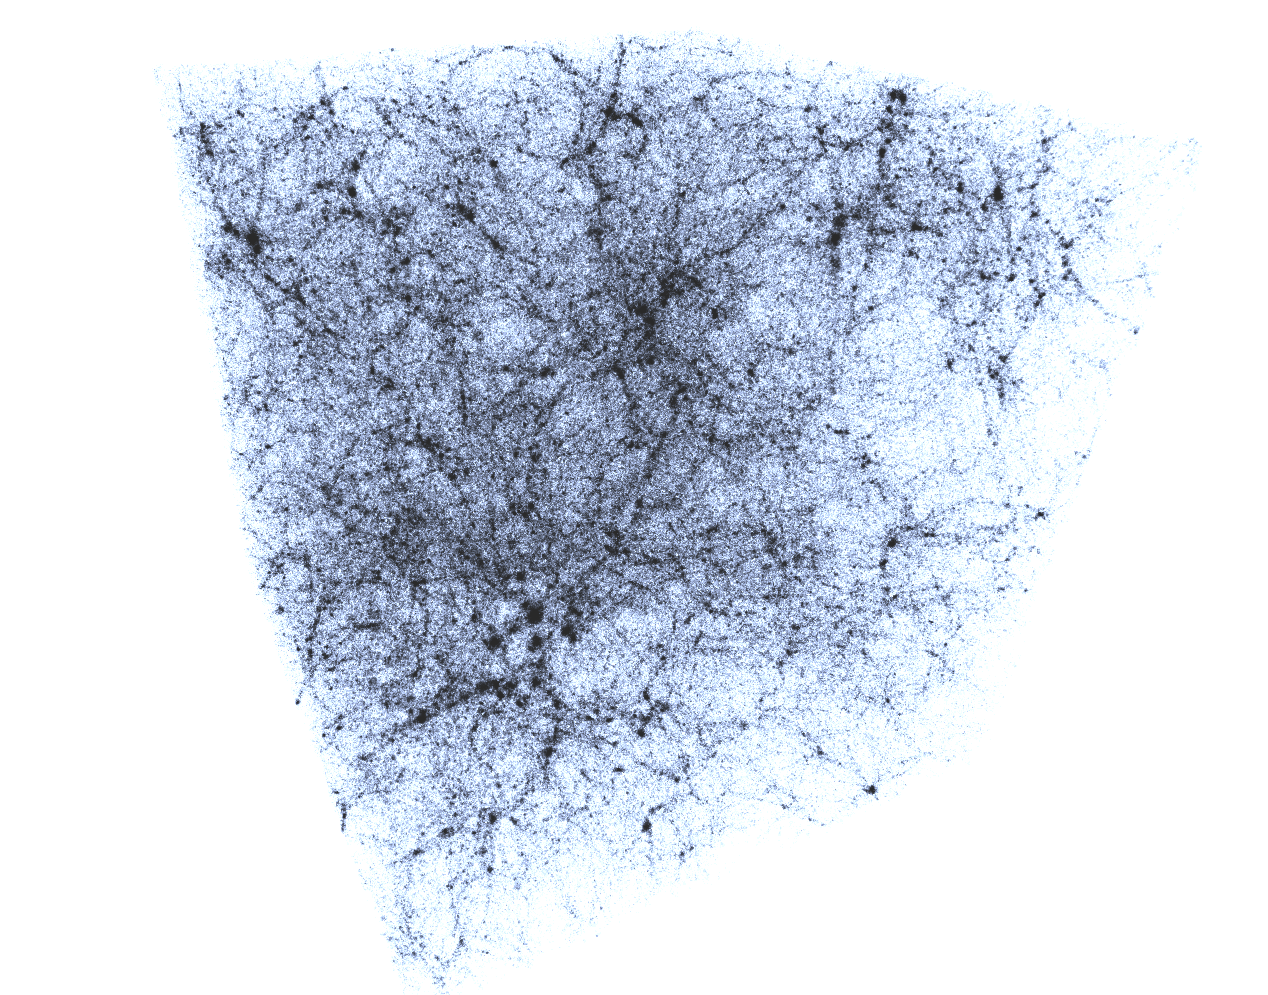
\includegraphics[width = \linewidth]{Figures/Chapter1/DMStruct.png}
    \caption{A visualization of the `cosmic web'. The shading shows the distribution of dark matter. The darkest regions are the spherical `halos' between the halos extended filaments can be seen. Regions of note are the void in the upper right and the clusters in the top middle and lower left, initially the dark matter density field would have been similar to the microwave background but giga-years of collapse have accentuated small features into a large structure. Image Credit: C.Marsden using the galaxy and structure visualization code Astera processing the Bolshoi Planck dark matter simulation (https://astera.soton.ac.uk/).}
    \label{fig:DMStruct}
\end{figure}

%Halo Finders, Halo mass functions, Merger Trees and EPS formalism
In order to analyse complex dark matter simulations, several classifications have been developed to describe the dark matter haloes. Firstly, `virialised haloes' collections of dark matter particles\footnote{Note here a dark matter particle is a simulation element, often millions of solar masses, and not the theorised fundamental particle.} that are balanced in terms of their potential and kinetic energy, mathematically, 
\begin{equation}
    \langle T \rangle = -\frac{1}{2}\sum^{N}_{k=1}\langle \mathbf{F}_k \cdot \mathbf{r}_k \rangle.
\end{equation}
Secondly, from a structural point of view haloes can be defined by their over-density. 
Specifically, a halo is defined as a sphere containing a density of mass that is a set number times that of a defined average density. The average density definitions commonly used are defined by either the background\footnote{The average density of the Universe.} or critical\footnote{The density required such that the universe will not expand forever.} density.
For example $M_{200c}$ would be the mass of a halo where the halo is defined as the spherical region that is 200 times the critical density. To identify these regions a number of methods have been developed:

\begin{itemize}
    \item Bound Density Maximum: BDM classifies halo structure by defining a spherical overdensity threshold, e.g. $M_{200c}$, then removes particles that exceed the escape velocity of the halo mass \citep{Klypin1997Particle-MeshSimulations}.
    \item Friends of Friends: FOF uses a dark matter particle linking threshold, particles are `linked' together if they are closer than the threshold. One particle cannot be in two FOF groups simultaneously such that particle groups are unique \citep{Davis1985THEMATTER}.
    \item ROCKSTAR (Robust Overdensity Calculation using K-Space Topologically Adaptive Refinement): ROCKSTAR is a cutting-edge development of the FOF halo finders. Using a 6-dimensional phase space and a temporal dimension the structure and evolution of haloes are extracted from dark matter simulations \citep{Behroozi2011TheCores}.
\end{itemize}

Once equipped with a halo classification and an extraction tool a language and formalism to describe how these structures relate to one another is required. Hierarchical assembly predicts halo growth via accretion followed by cannibalisation of a smaller halo, this process is not instant and during this time the smaller halo is situated within the larger and can be referred to as a subhalo. Subhaloes then may contain further structure from smaller halos they have accreted. Thus there are different `orders' of halos: $0^{th}$ order or central halos, $1^{st}$ order or sub-halos whose parent is a $0^{th}$ order halo, $2^{nd}$ order or sub-halos whose parent is a $1^{st}$ order halo, and so on. Useful statistical descriptions of the haloes are the halo and subhalo mass functions. The halo mass function is defined as the number density of central haloes of a given mass per unit volume. The subhalo mass function has multiple definitions depending on the definition of subhalo each definition is useful to a different context. Firstly, one can define the global subhalo mass function, similarly to the halo mass function this is the number density of subhaloes at a given mass per unit volume. Secondly, one can define the subhalo mass function relative to a particular central host halo, which provides the number of subhaloes of a given mass ratio $M_{subhalo}/M_{central}$ one expects to be associated to a halo mass $M_{central}$. 


Once a subhalo has been accreted onto a central halo it begins the process of merging. As the subhalo orbits, it gradually loses mass to the parent halo due to tidal disruption. This process is called `stripping', initially the outer regions of the subhalo are stripped with the denser centre remaining for longer. Once a subhalo can no longer be resolved by the simulation, and it's mass indistinguishable from the parent halo's mass it is regarded as fully merged. Information on this process is learnt from using the aforementioned halo finders to track substructures between simulation snapshots. As this is a simulated result it is important to note that the simulation calibration, e.g. the number of particles and force softening, can strongly affect the timescale of subhalo disruption \cite{vandenBosch2018DarkDisruption}.

As the subhaloes are an evolving population, it is necessary to state which subhalo mass definition one is using:

\begin{itemize}
    \item Unevolved Subhalo Mass Function (USHMF): This mass function is the total number of subhaloes that have accreted onto a central halo over its entire history. The subhalo mass is defined at the point of accretion and is frozen at infall and no number density is ever lost. This mass function is useful for understanding the total accretion history of a halo.
    \item Unevolved Surviving Subhalo Mass Function (USSHMF): This mass function is the total number of subhaloes that reside in a halo at a given epoch. Subhaloes once accreted are frozen in mass, however, at the time when they would have fully merged are then considered removed from the count. This mass function is useful as it retains information about the infall masses and can be further categorised to retain information about number density contribution from different infall epochs.
    \item Evolved Subhalo Mass function (ESHMF): This mass function is the total number of subhaloes that reside in a halo at a given epoch where the subhaloes have undergone mass loss/transfer to the central halo. This mass function is the `true' subhalo mass function that one would expect to see if dark matter were directly testable e.g. via galaxy lensing in groups and clusters \cite{Bartelmann2001WeakLensing}.
\end{itemize}

In Figure \ref{fig:SubHaloes_byz}, in the left-hand panel we show the halo mass function at redshift $z=0.1$. Note the characteristic Schechter function shape with an inverse linear relationship between number density and halo mass in log-log space, which breaks and rapidly declines above a threshold mass, which at this redshift is roughly $M_h\sim 10^{14}$ $M_{\odot}$. In the right-hand panel, we show the Global Unevolved Surviving Subhalo Mass Function at redshift $z=0.1$. In both panels, the coloured shading represents the contribution to the global USSHMF at different redshifts of infall, note the logarithmic scaling means the shading is not linear. Recent accretion is the dominant contributor of subhaloes at all masses. Furthermore, high mass subhaloes $M_h \geq 10^{13} M_{\odot}$ accrete only at redshifts below $z < 2$.

\begin{figure}[h]
    \centering
    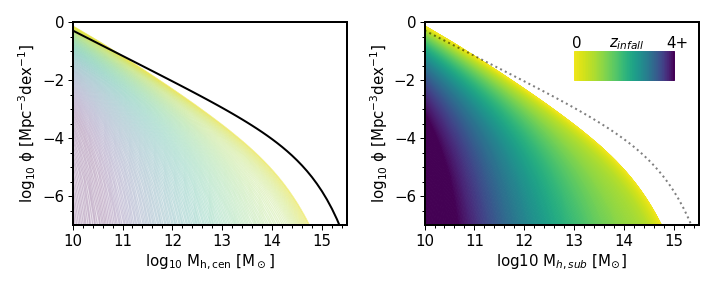
\includegraphics[width = \linewidth]{Figures/Chapter1/SubHaloes_byz.png}
    \caption{Left: Central Halo Mass function, the global number density of haloes at redshift $z=0.1$. Right: Global Unevolved Surviving Subhalo Mass Function at redshift $z=0.1$. The colour gradient shows the fraction of subhaloes at each mass coloured by the redshift of infall. Note due to the logarithmic scaling the thinner yellow bar at the top of the distribution is a majority contribution of subhaloes, showing that at all masses recent accretion dominates the population.}
    \label{fig:SubHaloes_byz}
\end{figure}

In addition to the distinction between central and satellite haloes, information about the full mass assembly is also extracted from simulations. Halo assembly histories are commonly visualised as simple(\textit{ish}) tree networks, referred to as a ``merger trees''. Central haloes are identified at a low redshift and the main progenitors followed backwards in time to create the central `trunk'. At any epoch where a merger occurs, the main progenitor is assigned to be the larger of the two merging haloes\footnote{This remains true even if the main progenitor branch becomes smaller than the other branch at an earlier redshift.}. At each merger a `branch' is created following this branch which followed back in time gives the assembly history of that halo. We show an example of a simple merger tree in Figure \ref{fig:SimpleTree}.

\begin{figure}[h]
    \centering
    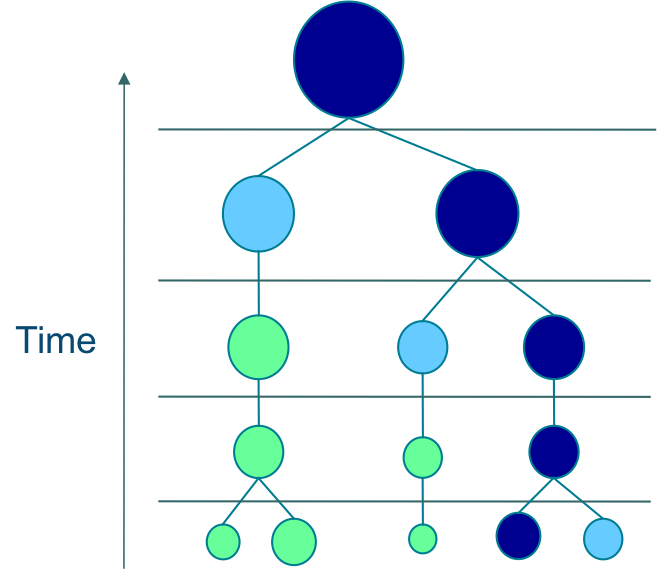
\includegraphics[width = \linewidth]{Figures/Chapter1/Merger_Tree_Simple.png}
    \caption{A cartoon of a simple merger tree. Increasing time moves up the page as indicated on the right, horizontal lines separate epochs. Dark blue circles represent the main progenitor or trunk haloes of the merger tree. Haloes that merge directly onto the trunk are coloured in light blue, the merger history or branch for each of these merging haloes is shown in green.}
    \label{fig:SimpleTree}
\end{figure}

There are increasingly more complex merger tree diagrams, it is not the case that a haloes merge simply we list some examples and show what these may look like on a stylised merger tree in Figure \ref{fig:Substructures}.

\begin{itemize}
    \item Substructure: A halo is not immediately dissolved upon accretion to the central halo, the substructure is therefore maintained in central haloes between epochs. Furthermore, haloes on accretion may also carry internal substructure, which creates 2nd (and above) order substructure in the parent halo.
    \item Flyby Haloes: Some haloes may pass through another halo and may lose mass but are not captured. These haloes are known as flyby halos and must be accounted for when constructing mass functions to not inflate the number count of subhaloes.
    \item Re-Accreted Haloes: Haloes on particularly eccentric orbits or haloes with initially high velocity may enter a halo subsequently leave the halo group. These haloes whilst still bound to the group may not be associated with the group by a halo finder appearing to be flyby haloes. However, they at some later may reenter the group: Firstly, one must ensure these halos are not double-counted. Secondly it caution must be taken the mass they are accreted at is fit for purpose (i.e., mass at last accretion, mass at first accretion, or peak mass).
\end{itemize}

\begin{figure}[h]
    \centering
    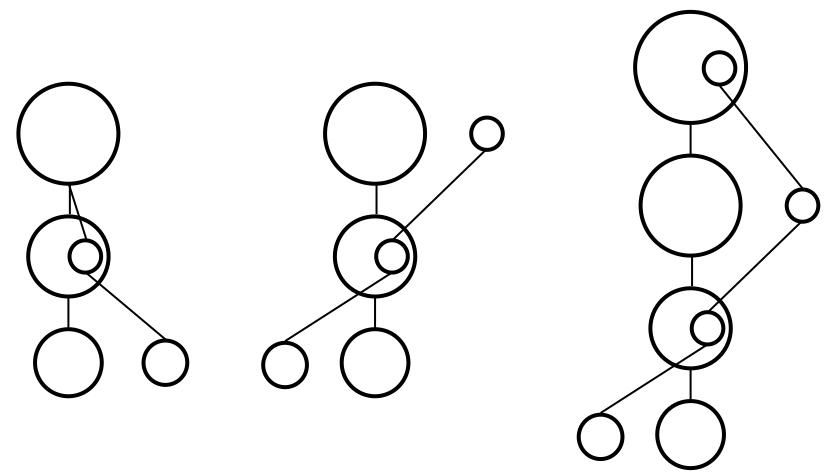
\includegraphics[width = \linewidth]{Figures/Chapter1/Substructures.png}
    \caption{From left to right: An example of: $1^{st}$ order substructure, a flyby halo and, a re-accreted halo.}
    \label{fig:Substructures}
\end{figure}

Whilst there is clearly a wealth of information available from dark matter simulations they are costly require a large amount of computational power both to run and analyse. For many models of galaxy evolution the information provided is far in excess of what is required. Press-Schechter Formalism \citep{Press1974} provides an alternative way to generate simple analytic dark matter distributions at a greatly reduced computational cost. For a simple visualisation, one can consider the dark matter distribution at high redshift as a random Gaussian probability distribution. 


Peaks in this distribution represent dark matter overdensities which will collapse over time where higher peaks collapse earlier due to greater gravitational influence. This can be visualised as a time-evolving threshold above which the dark matter density would qualify as a collapsed halo. If the summation of two Gaussian distributions are above this threshold then they become a single over-density or halo. A simplified cartoon is shown to visualise this in Figure \ref{fig:PS_Cartoon}.

\begin{figure}[h]
    \centering
    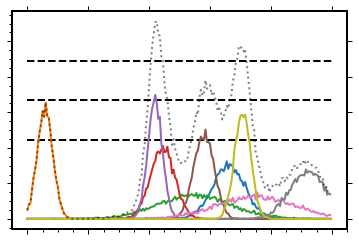
\includegraphics[width = \linewidth]{Figures/Chapter1/PS_Cartoon.png}
    \caption{A visualisation of the core theory of Press-Schechter Formalism. The solid coloured lines are random Gaussian distributions representing fluctuations in the initial mass density field, the grey dotted line is the total mass distribution. The three black dashed lines are for visualising the threshold of collapse at different epochs. The x-axis is an arbitrary spatial dimension, and the y-axis an arbitrary density unit.}
    \label{fig:PS_Cartoon}
\end{figure}

Following Figure \ref{fig:PS_Cartoon} considering the top dashed line as the earliest epoch we look for collapsed haloes by examining the dashed line; two peaks in the density field can be found above the threshold denoting two collapsed halo structures. The area above the threshold is analogous to the mass of the halo and the spread of the peak analogous to the size. At the second threshold, there is another collapsed peak mostly contributed by the brown Gaussian. Furthermore, the two peaks from the first collapse have grown in mass as can be seen by an increased area and spatial extent. Finally, looking at the last collapse threshold: On the left, there is a new isolated peak; on the right, the peaks created by the yellow and brown Gaussian distributions now create one continuous area above the threshold, this is an indication of two merged haloes. Within this merged halo, there are two distinct peaks that can indicate the nature of the halo substructure. It evident that at later epochs the merged substructures will also include the purple peak. This picture is an oversimplification of Press-Schechter Formalism, the Gaussian field is actually significantly more interesting the density fluctuations mirror the distribution of the cosmic microwave background. Furthermore, instead of simple collapse thresholds, a window function is used to smooth the density field. Finally, here the peaks are represented as static, however, their size and location will evolve with time. The shift in the location of the peaks can be used to build dynamic halo histories without the need for full N-Body simulations \cite{Voivodic2019ExcursionCatalogues}.

The Press-Schechter Formalism can be used to analytically create a merger tree by utilising the probability of any two overdensities merging. An algorithm that starting at a given redshift with a given halo mass can then construct a theoretically valid merger history. We summarise here the \textsc{galform} \citep{Cole2000} algorithm for making merger trees from Press-Schechter Formalism\footnote{In \citet{Parkinson2008GeneratingTrees} improvements to this method are proposed to better align the generated merger trees with the millennium simulation by using a perturbing function to remove systematic differences between N-Body simulations and the algorithm.}.

\begin{itemize}
    \item Pick a starting Mass, $M_{h}$ and redshift $z$. This will be the final mass/redshift for the main progenitor halo in the tree.
    \item Step backwards in redshift in steps, $dz$, where $dz$ is chosen that the probability, $P$, of a halo having a merger in $dz$ is $P\ll1$.
    \item Generate a uniform random number, $N$, if $N<P$ the halo splits, else the mass is reduced to account for unresolved haloes or smooth accretion and the process repeats.
    \item If the halo has split a random number is generated from the probability distribution that defines the possible progenitor halo masses from  Press-Schechter Formalism this is the mass of the split halo, $M_{split}$. The central halo mass is then updated to be less the split mass and a smooth/unresolved accretion component and the process repeated.
\end{itemize}

The merger trees generated using this algorithm are simpler and less computationally expensive than those extracted from N-Body simulations, and if calibrated properly fully consistent with \LCDM cosmology. They, therefore, are an ideal choice for simulations that need to generate halo merger trees on demand.

\section{Hydrodynamic and N-Body Simulations}
\label{sec:Hydro}
%What is Hydrodynamics or N body
Hydrodynamical simulations are the most physical galaxy models simultaneously simulating baryons and dark matter. Within a volume dark matter, gas, and stars are assigned to particles and/or grid cells. Forces between particles are then applied to each element with respect to other elements. The volume is then advanced by repeated numerical solving and time stepping. At set intervals, snapshots are produced to be used for analysis. Processes that take place below the resolution limit of the simulation, such as star formation, are simulated using a sub-grid analytic routines based on the properties of the given volume element.

%State of the Art
\subsection{State of the art: Illustris TNG}
The Illustris TNG simulations are a suite of 18 simulations, which use three different volumes, $\sim 50, 100, 300$ ${Mpc}^{3}$, and include a range of physical processes and resolutions. TNG at its core uses the code \textsc{arepo} \citep{Springel2010EMesh}, a mesh-based code, which solves coupled ideal magneto-hydrodynamics and self-gravity using periodic boundary conditions. Even for TNG50, where exceptionally high resolution is achieved, much of the baryonic physics falls below the resolution limit, thus relying on `sub-grid' models. Sub-Grid models are used for star formation, feeding of supermassive black holes, galaxy feedback process (star formation and AGN), and more. A specific example of one such sub-grid model is star formation: Gas above a threshold density of $n_H \simeq 0.1cm^{-3}$ is allowed to form stars following the numerical results of \citet{Springel2003CosmologicalFormation}. Sub-grid models attempt to replicate results of smaller higher resolution simulations or from observations. 

%Drawbacks
\subsection{Pros and Cons}
The drawbacks of using a hydrodynamic model are foremost limitations of resources. They require vast amounts of computational resource to run and take a lot of developer time and skill to create. Furthermore, they create huge amounts of output data that can be difficult to process and interpret. Last but not least all simulations are subject to volume and resolution constraints. For example, the TNG simulations run three box sizes; the larger boxes can simulate rare/low abundance objects, whereas, the smaller boxes can simulate galaxies in high detail. The computational time to run a simulation that produces both high detail and rare objects would make the computational cost impractical and the data products unmanageable with current tools and technologies. 

The advantages of explicitly modelling galaxies using hydrodynamics is that one can study the dynamics and interactions of the particles pertaining to each galaxy or dark matter halo directly. Furthermore, by carefully choosing the size and resolution of the simulation, it is possible to probe the connection between large and small scale structures over many orders of magnitude. For example, in TNG it is possible to explore how the cosmological environment affects galaxy formation, the gas flow along dark matter filaments and, the statistics of galaxy mergers. 
Alternately in FIRE \cite{Hopkins2018FIRE-2Formation}, an advanced smooth particle hydrodynamic simulation, one high resolution `zoom in' region is simulated with high fidelity. The particle resolution in FIRE is such that feedback from star formation winds, AGN, and even individual supernovae are resolved. Hydrodynamics represent the stare of the art in our ability to simulate a universe or an individual galaxy holistically. However, the high computational and human cost associated with their running and development means they are not the ideal tool for rapid testing of new theories or ideas. 

Progress has been made in each aspect that limits hydrodynamics. Firstly, the speed, memory and architecture of computing resources continue to improve with recent advances in GPU technology contributing to the overall power available to simulators. In addition to this, novel techniques have been developed such as ``genetic modification'', whereby the initial conditions of a simulation are subtly altered to test how perturbations and modelling assumptions affect self-similar galaxies \citep{Pontzen2017HowGalaxy}. Building on these advances in speed and flexibility it may well become possible to use hydrodynamic simulations as comprehensive tools. At present we must still utilise diverse sets of complementary tools available to deal with the highly non-linear and complex processes regulating galaxy formation and evolution.

\section{Semi-Analytic Modelling}
\label{sec:SAM}
%What is a SAM
\subsection{History of Semi-Analytic Models}
Building off the hierarchical collapse models from \LCDM cosmology and the power of generating merger trees from EPS routines \citep{Press1974}, a new form of galaxy model was conceived named semi-analytic models. The dark-universe, e.g. dark matter, was conceived of from the rotation curves of galaxies, it follows that galaxies must be influenced by the structure formation of the dark matter haloes predicted by \LCDM cosmology. The earliest models successfully recreated the galaxy luminosity function by assigning the baryonic matter to EPS haloes and solving analytic gas collapse equations \citep{White1978CoreClustering}.

%Brief aside on the simple analytics here?

Semi-analytic models were then developed and extended to include more advanced galaxy physics, such as the formation of galaxy disks \citep{Mo1998TheDiscs}. Increasing in complexity by both folding in more advanced physics such as AGN feedback and using merger trees from N-body dark matter simulations the models were able to increase the scope of predictions by tuning parameters over several simulation runs to best fit the observations \citep{Bower2006BreakingFormation}. Continuing improvements in cosmological (dark matter) simulations have allowed for semi-analytic models to improve both in resolution and size. In addition, as computing power has become more accessible and better improved Monte Carlo methods have been developed, this has allowed for the development of a variety of multi-parameter semi-analytic models tuned over hundreds of thousands of runs \citep{Guo2011FromCosmology,DeLucia2011TimesCosmology,Fontanot2011TheUniverse,Menci2014TriggeringInteractions,Somerville2015StarGas}.
In this section we will discuss the state of the art in semi-analytic modelling by summarising a review by \citet{Somerville2015StarGas}, followed by deconstructing a subset of the latest models, and finally, present a consideration the drawbacks of semi-analytic models compared to other galaxy modelling techniques.

\subsubsection{Somerville (2015) Review \citep{Somerville2015StarGas}}
\textit{The semi-analytic models used here have been described in detail in Somerville \& Primack (1999), Somerville et al. (2001) and most recently in Somerville et al. (2008a, hereafter S08) and Somerville et al. (2012, S12). The Santa Cruz modelling framework has also recently been described in Porter et al. (2014). We refer the reader to those papers for details.}

This review explores three models published in \citet{Somerville2008ANuclei} (hereafter S08), \citet{Somerville2012GalaxyObservations} (hereafter S12), \citet{Porter2014ModellingSpace} (hereafter Santa Cruz). Each of these models is run using EPS merger trees as a backbone. Using analytic merger trees allows for high-resolution simulation reducing the minimum halo size. Reducing the halo size, in turn, allows the simulation of smaller galaxies. Galaxies grow via the cooling of gas from re-ionisation. Before this point haloes are seeded with gas at the cosmic baryon fraction. After this gas cools as given in \cite{White1991GalaxyClustering}, it condenses and forms stars at the centre of dark matter haloes. 

The prescriptions made to handle the hierarchical assembly predicted by \LCDM cosmology concern firstly the halo structures. At the point of halo merger, the larger halo and associated galaxy are assigned as the central, the smaller halo(es) and associated galaxies become subhaloes and satellite galaxies. Satellite galaxies then merge with the central galaxies on timescales given by the Chandrasekhar formula \citep{Chandrasekhar1943DYNAMICALFRICTION}, as given in, for example, \citet[e.g.][]{Boylan-Kolchin2008}. The mergers of satellites are one of the methods that transform the morphologies of central galaxies, mergers gradually reduce the central galaxies angular momentum eventually creating a spheroid \cite{Hopkins2009HOWMERGERS}. 

In addition to changing the morphologies of central galaxies, mergers are also thought to drive one of the two pathways of star formation. During a merger as the gas of the two merging galaxies is destabilised triggering fragmentation and a galaxy-wide starburst, a short period where star formation is enhanced by up to an order of magnitude \citep{Hopkins2009HOWMERGERS}. The second mode of star formation is referred to as ``disk mode'' and is usually modelled in three ways: The Kennicutt-Schmitt law \citep{KennicuttJr.1998TheGalaxies} assumes that the surface density of star formation, $\Sigma_{SFR}$, is related to the surface density of cold neutral gas, $\Sigma_{gas}$,

\begin{equation}
    \Sigma_{SFR} = A_{SF}\Sigma_{gas}^{N_{SF}}.
\end{equation}

It is here and in the following star formation rate recipes that the first tuning parameters are found; $A_{SF}$ and $N_{SF}$ control respectively the normalisation and slope of the star formation rate law. In addition there are two critical gas densities $\Sigma_{crit}$ and $\Sigma_{H2,crit}$, below which neutral gas or molecular gas will not form stars. Similar to the Kennicutt Schmitt recipe, molecular gas star formation follows empirical results that link the molecular gas surface density to the star formation rate as empirically determined by \citet{Bigiel2008TheResolution},

\begin{equation}
    \Sigma_{\mathrm{SFR}}=\left(\frac{A_{\mathrm{SF}}}{10 M_{\odot \mathrm{PC}^{-2}}}\right) \Sigma_{\mathrm{H}_{2}} N_{\mathrm{SF}}.
\end{equation}

Its observed that above a critical H2 density the SFR steepens \citep{Narayanan2012ALaw}, inspired by this the SFR may also be modelled using a two part scaling law, 

\begin{equation}
    \Sigma_{\mathrm{SFR}}=A_{\mathrm{SF}}\left(\frac{\Sigma_{\mathrm{H}_{2}}}{10 M_{\odot \mathrm{pc}^{-2}}}\right)\left(1+\frac{\Sigma_{H_{2}}}{\Sigma_{\mathrm{H}_{2}, \mathrm{crit}}}\right)^{N_{\mathrm{SP}}}.
\end{equation}

Semi-analytic models rely on several feedback prescriptions to regulate their star formation. The energy released during supernovae, created as a result of star formation is deposited in the inter stellar medium consequently driving outflows of cold gas at the rate,

\begin{equation}
    \dot{m}_{\mathrm{out}}=\epsilon_{\mathrm{SN}}\left(\frac{V_{0}}{V_{c}}\right)^{\alpha_{\mathrm{rh}}} \dot{m}_{*}.
\end{equation}

Where $\epsilon_{\mathrm{SN}}$ is a parameter that scales the efficiency of the supernovae's ability to drive outflows, and the remaining parameters control the binding properties of the gas. In addition to supernova feedback, most SAMs include AGN feedback caused by energy/momentum release from the supermassive black hole at the centre of the galaxy. AGN feedback is believed to act in two distinct modes: The first mode, ``quasar mode'', is initiated after a galaxy merger, as the black hole grows in mass, more energy is released to the ISM until the gas accretion is halted by outflows from the black hole. In this mode, AGN feedback gradually reduces the SFR by heating the cold gas reservoir. The second AGN feedback mode, ``radio mode'', is commonly assumed to be in the form of a jet and triggered when accretion drops below a few per cent Eddington. This feedback can also prevent late cooling gas in the central regions of galaxies \cite{Croton2007Thequenching}.

The takeaway of this brief introduction to semi-analytic modelling is that they can be characterised by heavy parametrisation of each singular observable which results in a very highly parameterised model. This is due to the large uncertainties in the choice (and strength thereof) of the physical processes to include. The interested reader can find additional semi-analytic methods that control the properties of the gas described in Appendix \ref{Appx:ExtraSAM}. The following subsections will describe two state of the art semi-analytic models.

%State of the art SAM
\subsection{State of the art}
Many of the modern semi-analytic models many were conceived in the mid-two-thousands and have been iterated on for over a decade, due to increasing complexity without significantly improving convergence in results thus they are arguably reaching a plateau in usefulness. During this time the amount, quality and availability of comparison data have significantly increased. As the models have matured they have been continually added to with many physical prescriptions to match a wide variety of observations, although many still struggle to reproduce the basics of galaxy evolution such as the evolution of the stellar mass function \cite{Asquith2018CosmicModels}. Here we briefly discuss two models that represent state-of-the-art in semi-analytic galaxy modelling.

\subsubsection{GAEA}
%Hirschmann2016GalaxyModel
The GAEA model is a good example of a mature semi-analytic model, originating from the seminal work modelling assembly of BCGs by \citet{DeLucia2007TheGalaxies}. It has subsequently been updated many times in 2008 (De Lucia \& Helmi) 2010 (Li et al.) 2014 (De Lucia et al.) and \citet{Hirschmann2016GalaxyModel} (see references within).
%Zoldan2019TheEvolution
One of the latest renditions of this model based on that of \citep{Xie2017H2-basedFormation} and updated in \citep{Zoldan2019TheEvolution}, this version of the model includes a description of quasar driven winds in an effort to reproduce the size-mass relation for both early and late-type galaxies.

\subsubsection{SHARK}
%lagos 2018 Li et al.
%lagos 2019
The SHARK semi-analytic model represents an attempt to keep the field of semi-analytic models in line with current software engineering best practice. The release paper \citep{Lagos2018Shark:Formation} carefully details the physical prescriptions and modularity that defines the code. SHARK is designed to be flexible and modular and takes pride in being the most accessible open-source code available. In \citet{Lagos2018Shark:Formation} the authors show the baseline performance of SHARK to be as good as or exceeding other semi-analytic models in the mass-size, gas-stellar mass and stellar mass-metallicity relations. The flexibility of SHARK is then demonstrated in \citet{Lagos2019FromModel}, where  SHARK is modified to use different dust mass models to match spectral energy distribution observations of galaxy emission from the far-UV to the far-IR.

%Drawbacks of SAM
\subsection{Drawbacks of Semi-Analytic Modeling}
A major feature of a Semi-Analytic modelling is the number of parameters that can be tuned to reproduce observations, for example, the default SHARK configuration has over 50 input parameters included. Whilst the breadth of these parameters allows for semi-analytic models to produce fits to a wide range of observational properties, they also inevitably present serious degeneracies, thus obscuring the actual significance of the specific physical processes assumed in input \citep{Lapi2011DarkModels,Gonzalez2011Evolution4}.


\section{Semi-Empirical Modelling}
\label{sec:SEM}
%What is a SEM
Semi-empirical models similarly to semi-analytic models are often built on numerical or analytical dark matter merger trees \cite{Zavala2012}. A semi-empirical model uses a set of observations as inputs to build the model upon and another set of observations as an output. 
For example, many semi-empirical models us the stellar mass function to calibrate the mass and mass growth of galaxies. In brief, this is achieved by comparing the relative abundance of dark matter haloes and observed galaxies. Under the assumption that galaxies reside in parent halos that share a similar number density an analytic correlation between halo mass and stellar mass is determined \citep{Kravtsov2004TheDistribution,Shankar2006NewFormation}. This process is called abundance matching and is explained in greater depth in Section \ref{C2:SubSec:AbnMtch}. When used correctly abundance matching ensures that semi-empirical models recreate the observed distributions of galaxies over many redshift epochs. By then using the growth of dark matter haloes merger trees and the abundance matching relation the need for modelling of galaxy mass and growth is removed via this empirical constraint. Constraining galaxy masses and/or other properties via observations significantly reduces the modelling parameter space compared to hydro-dynamical or semi-analytic models. A reduced parameter space increases the transparency of the model by making the effects of the other parameters more clear. By empirically fixing properties that may not yet have clear constraint or physical mechanism, or those properties that are not of interest to the current simulation, semi-empirical models are able to focus on the reproduction of a singular or small subset of properties.

Since there inception, semi-empirical models have grown in complexity and in doing so have naturally increased the number of modelling parameters. However, as the complexity of the models is controlled by observational priors and the model should be \textit{internally consistent}, and thus it is possible to accurately probe very specific aspects of galaxy formation. It is, however, possible to create SEM where the observational priors, and by extension the model, are \textit{internally inconsistent} i.e. one or more of the observational inputs do not agree. An example of such inconsistency can be has been found in observed stellar mass function and the observed star formation rate. The time integral of the star formation rate predicts far more stellar mass growth than is possible with the observed growth of the stellar mass function \citep{Leja2015ReconcilingFunction,Lapi2017StellarEquation}. If these two empirical properties were included in a semi-empirical model then the model would be \textit{internally inconsistent}. However, the semi-empirical model could use the stellar mass function as an input to show the implied star formation rate without needing the conflicting measurement to form a physical part of the model. Similar yet unappreciated effects involving systematics in galaxy assembly make up a significant part of Chapters \ref{Chapter:GalGrowth} \& \ref{Chapter:GalPairs}.

\subsection{State of the art}
Here we describe three state-of-the-art semi-empirical models. Each of the models described here has a radically different approach to semi-empirical modelling. They are each constrained by observational priors and make predictions about the buildup of mass in galaxies through mergers and star formation rate. The range of approaches show the flexibility and the agreement between models show the power of the empirical approach. 


\subsubsection{\citet{Rodriguez-Puebla2017ConstrainingProperties}}
%Aldo
In the model presented in \citet{Rodriguez-Puebla2017ConstrainingProperties}, the SMHM is constrained using the 2 point correlation function and the evolution of the SMF. Using these constraints the inconsistency between observed SFR and SMF evolution is avoided. The main result of this paper is valuable constraints on the SFR and quenched fraction of galaxies in multi-parameter space, in both halo mass - redshift space and stellar mass - redshift space as shown in Figure \ref{fig:RP_fig}.

%Figure
\begin{figure}[h]
    \centering
    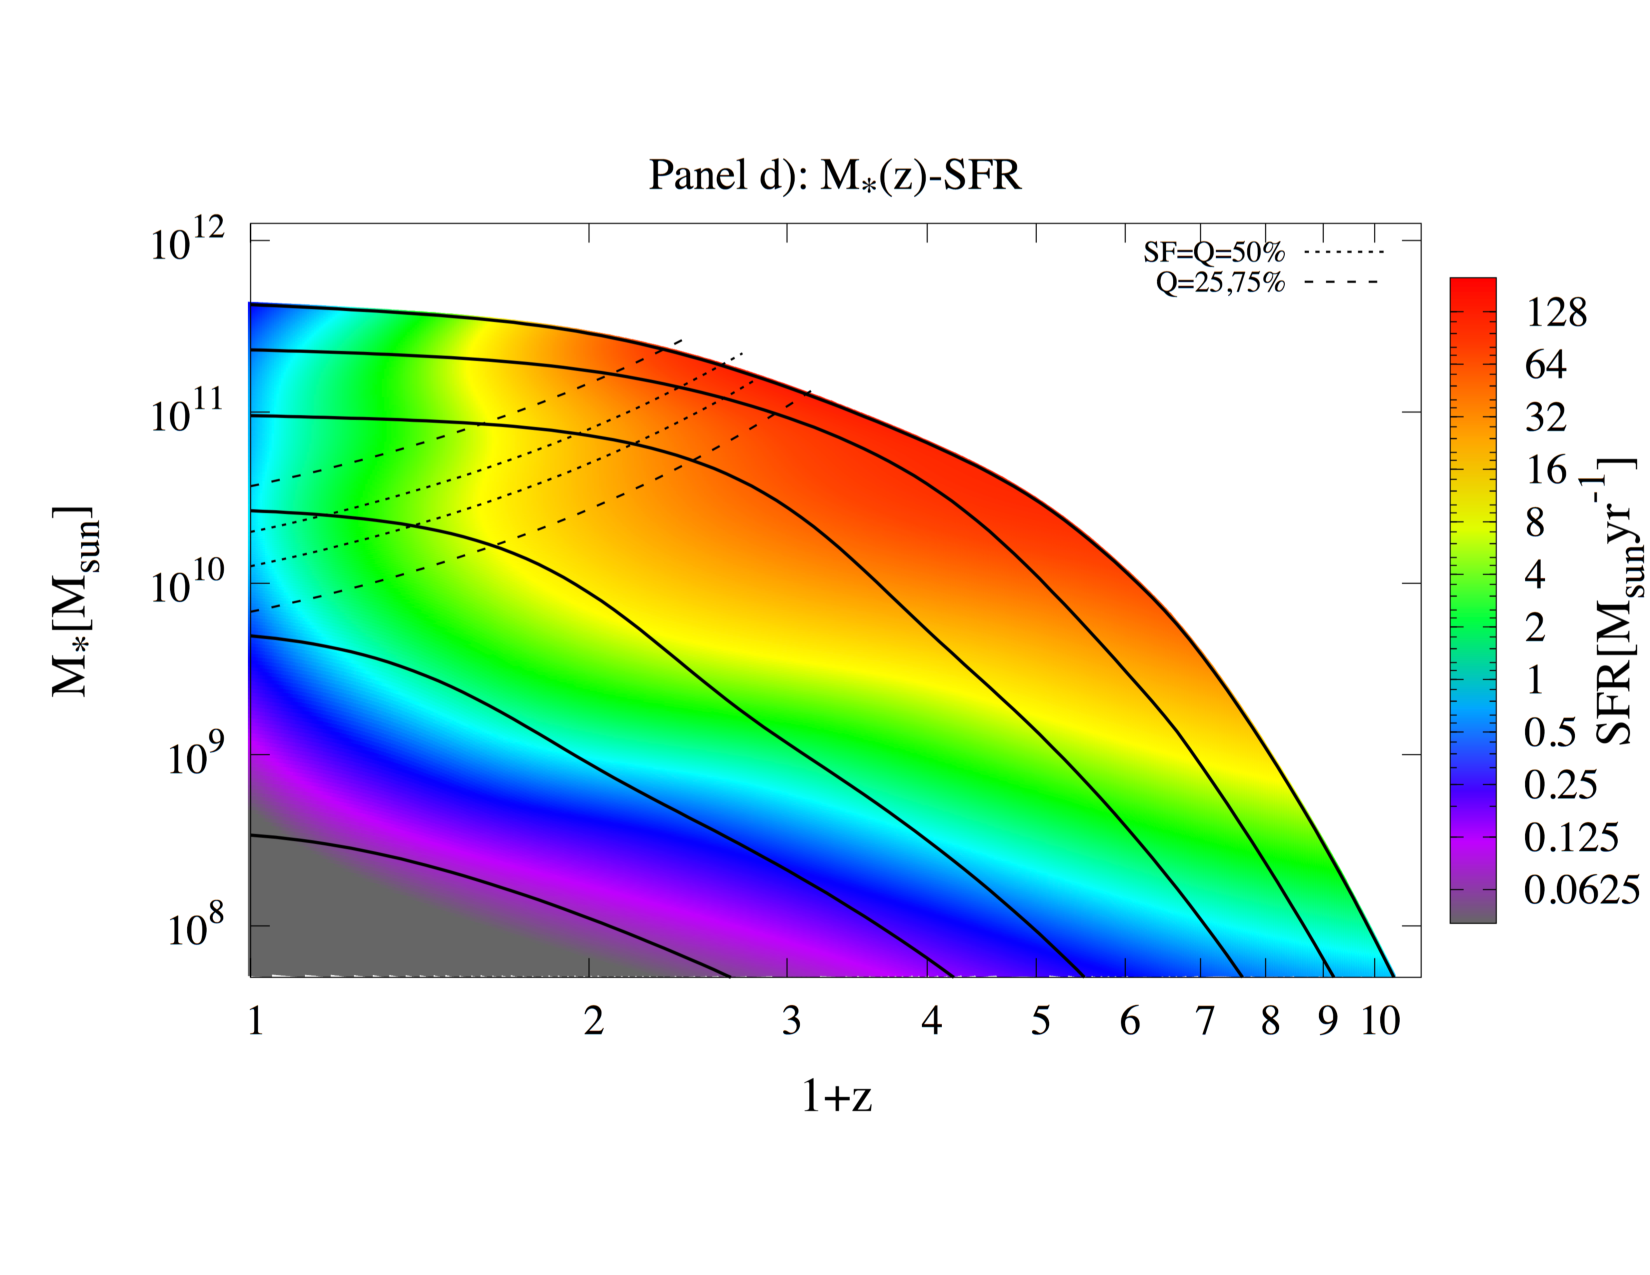
\includegraphics[width = \linewidth]{Figures/Chapter1/RP17_fig9.pdf}
    \caption{In this figure, the relationship between mass redshift and the star formation rate is shown. The black lines show the `galaxy mass tracks' the average path of the galaxies through $M_*$-z space. The colour shows the star formation rate associated with an average galaxy at that point in $M_*$-z space. The dotted and dashed lines show the location where a percentage of galaxies (as labelled) have been quenched.
    Image is used with permission from: Aldo Rodriguez Puebla \cite{Rodriguez-Puebla2017ConstrainingProperties}}
    \label{fig:RP_fig}
\end{figure}


The key message from \ref{fig:RP_fig} is that most stellar mass is built up ``in-situ'' at high redshift as the mass growth below redshift $z<1$ is a few per cent. In \citet{Rodriguez-Puebla2017ConstrainingProperties} it is also shown that massive galaxies then quench at the point where the sSFR is equal to the specific halo mass accretion rate which happens at $M_{vir} \sim 2 x 10^{11} M_{\odot}$, this point is shown on the figure as the dotted/dashed lines where it can be seen that the SFR rapidly decreases.


\subsubsection{E\textsc{merge}}
%Moster Emerge
E\textsc{merge}, presented in \citet{Moster2018Emerge10}, builds upon N-body dark matter simulations. From the dark matter simulation each halo is tracked with its growth history and relation to other haloes. E\textsc{merge} works under the core assumption that galaxies grow in conjunction with the dark matter haloes they reside in. This is achieved through coupling the star formation rate of each galaxy to the accretion rate of the host dark matter halo parameterised in the following way,

\begin{equation}
\begin{aligned} \log _{10} M_{1}(z) &=M_{0}+M_{z}(1-a)=M_{0}+M_{z} \frac{z}{z+1}, \\ \epsilon_{\mathrm{N}}(z) &=\epsilon_{0}+\epsilon_{z}(1-a)=\epsilon_{0}+\epsilon_{z} \frac{z}{z+1}, \\ \beta(z) &=\beta_{0}+\beta_{z}(1-a)=\beta_{0}+\beta_{z} \frac{z}{z+1}, \\ \gamma(z) &=\gamma_{0}, \end{aligned}
\end{equation}

where $M$, $\epsilon_{\mathrm{N}}$, $\beta$ and $\gamma$ are respectively the characteristic mass, efficiency normalisation, low mass slope and high mass slope. Each parameter has a value at redshift zero given by, e.g. $M_{0}$, and, with the exception of $\gamma$, a redshift evolution coefficient given by, e.g. $M_{0}$. Additional parameters are included controlling for example; the point at which satellite galaxies are disrupted returning all mass to the ICM, the fraction of mass ejected to the ICM during a merger, and quenching parameters from \citet{Wetzel2013GalaxyUniverse}, e.t.c. The fractions of `in-situ' vs `ex-situ' mass build up are computed and fit by,

\begin{equation}
f_{\mathrm{acc}}(z) =f_{2} \exp \left[-f_{1}(z+1)\right] 
\end{equation}

as well as the star formation histories that are fit by,

\begin{equation}
\log \Psi(z) =-\log \left[\Psi_{1}(z+1)^{-\Psi_{2}}+\mathrm{e}^{\Psi_{3}(z+1)-\Psi_{4}}\right] 
\end{equation}.

Similarly to \citet{Rodriguez-Puebla2017ConstrainingProperties} it is found that stellar mass is built up in-situ until a breakpoint at $1.1 \multiply 10^{12} M_{\odot}$. Above this point, larger galaxies may then accrete a significant proportion of their mass.

\subsubsection{U\textsc{niverse}M\textsc{achine}}
%Behroozi UnivM
U\textsc{niverse}M\textsc{achine} \cite{Behroozi2019UniverseMachine:010} is built on a background of halo merger trees extracted from the Bolshoi simulation \citep{Klypin2016,Rodriguez-Puebla2016HaloSimulations}, using the \textsc{rockstar} halo finder and the C\textsc{onsistent} T\textsc{rees} codes \cite{Behroozi2011TheCores, Behroozi2013GRAVITATIONALLYCOSMOLOGY}. There are 21 modelled outputs with 44 tuning parameters and 6 priors. Using a Markov Chain Monte Carlo the parameters are fit to a large set of observations though the algorithm depicted in Figure \ref{fig:BehMeth}.

%go to here for the source https://arxiv.org/format/1806.07893
\begin{figure}[h]
    \centering
    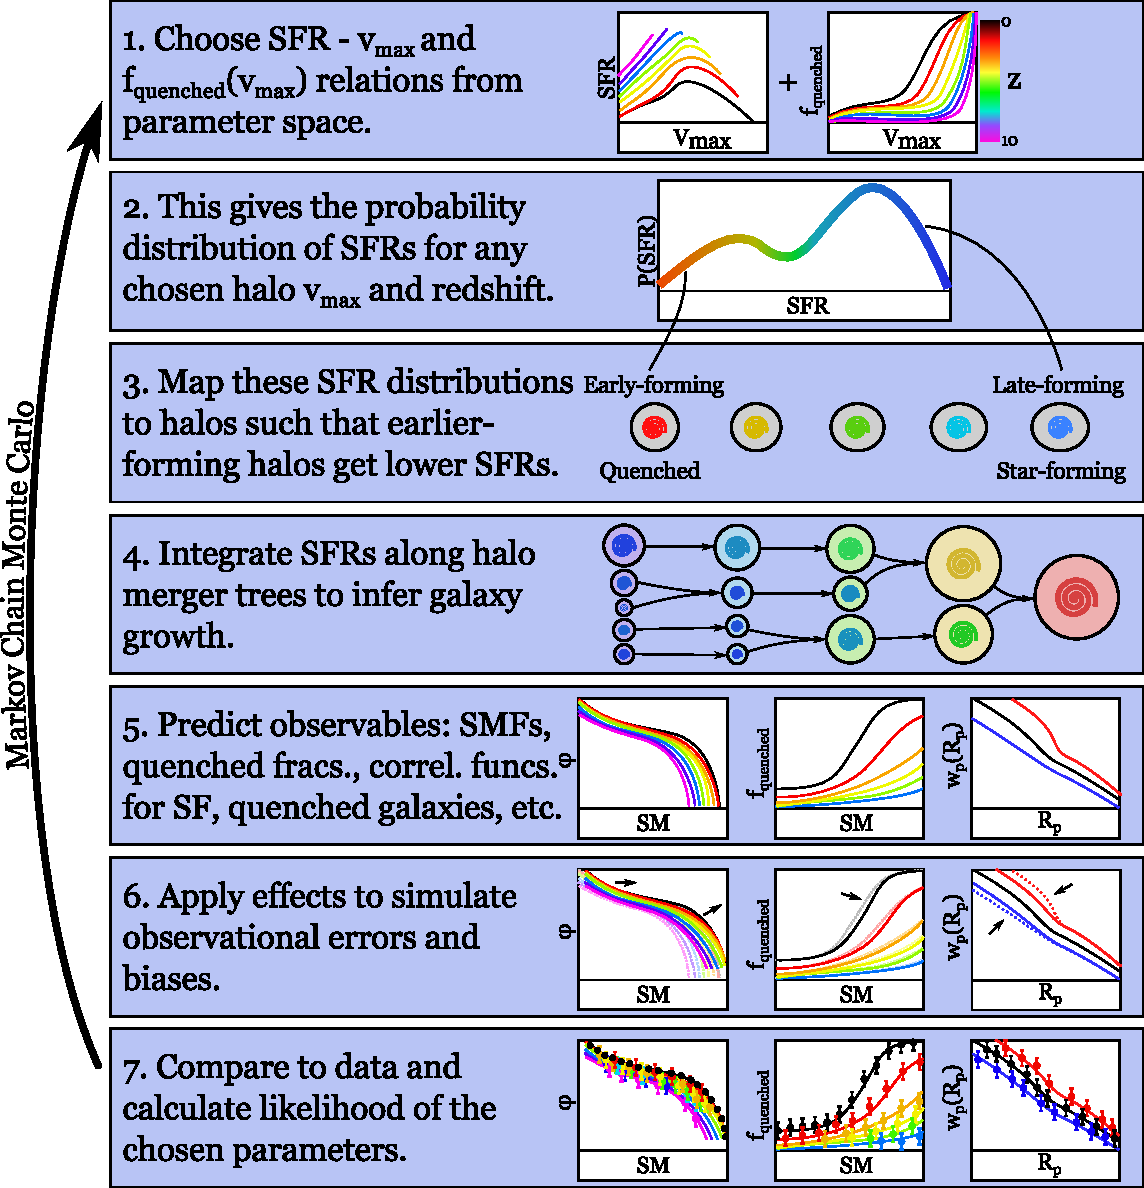
\includegraphics[width = \linewidth]{Figures/Chapter1/sfr_method.pdf}
    \caption{
    This figure shows the iterative process used by the Markov Chain Monte Carlo in U\textsc{niverse}M\textsc{achine}. As described by the labels in the figure relations from the empirical parameter space are chosen (1), giving a SFR distribution (2). The distribution is mapped into haloes (3), the SFR is integrated along the merger histories to infer the galaxy growth (4). Observable features are produced (5), and observational bias corrections applied (6). Finally, this is compared to the data and the likely-hood of the parameters produced and new parameters picked accordingly.
    Image used with permission from: Peter Behroozi \cite{Behroozi2019UniverseMachine:010}}
    \label{fig:BehMeth}
\end{figure}

U\textsc{niverse}M\textsc{achine} works by iterating over three key steps:
\begin{itemize}
    \item Parameter selection and probability distribution generation. This step phase samples a subsection of the parameter space and computes the associated star formation probabilities that exist within it. (Fig. \ref{fig:BehMeth}: 1 \& 2)
    \item Mapping into and integration along halo merger trees. The SFR distributions are mapped into haloes then using the halo merger trees integrated forward though time to estimate central galaxy mass. (Fig. \ref{fig:BehMeth}: 3 \& 4)
    \item Observable simulation. A set of observables are then extracted from the galaxy population and given simulated observational errors. These are then compared to data and the likelihood of the parameters chosen in the first step calculated. (Fig. \ref{fig:BehMeth}: 5, 6, \& 7)
\end{itemize}

This model is massively parallel allowing for over $10^{5}$ cores involved in any given parameter estimation. The model predictions are numerous included in which are `in-situ' vs `ex-situ' growth ratios in broad agreement with the other models.

\subsection{Limitations of the empirical technique}
%Drawbacks of SEM
Semi-empirical models, as demonstrated above, come in many different flavours. Whilst data is what empowers semi-empirical models, it also presents one of semi-empirical models major limitations. Having wide and deep data sets which give statistically representative samples via large volumes to high redshift is difficult and costly. Most techniques involve correcting data sets and surveys to be consistent with one another creating a patchwork connecting the local and distant Universe. Semi-empirical models will continue to improve along with the available data. However, when built upon traditional dark matter simulations they will share the volume constraints found in semi-analytic and hydro-dynamical models.


\section{Galaxy Surveys Present and Future}
\label{sec:Surveys}
Galaxy surveys are the cornerstone of semi-empirical galaxy modelling. Combined with dark matter simulations they form the basis of abundance matching. Other properties such as star formation, colour, shape, size, position, e.t.c., can all form constraints for, either inputs or outputs, of semi-empirical models. It, therefore, stands that improving the quality of models is predicated on improving the quality of the data.

\subsection{Past and Ongoing Surveys}
The galaxy surveys essential to semi-empirical models come in two forms `wide' and `deep'. Wide surveys look to cover a large area of the sky to get a statistically significant sample of the galaxy population. Deep surveys cover a much smaller area but use longer exposures to observe much fainter objects. The trade-off between width and depth is visualised by a simple example in Figure \ref{fig:WvD}. Tight surveys collect more photons per unit area and can, therefore, see to a greater depth.

\begin{figure}[h]
    \centering
    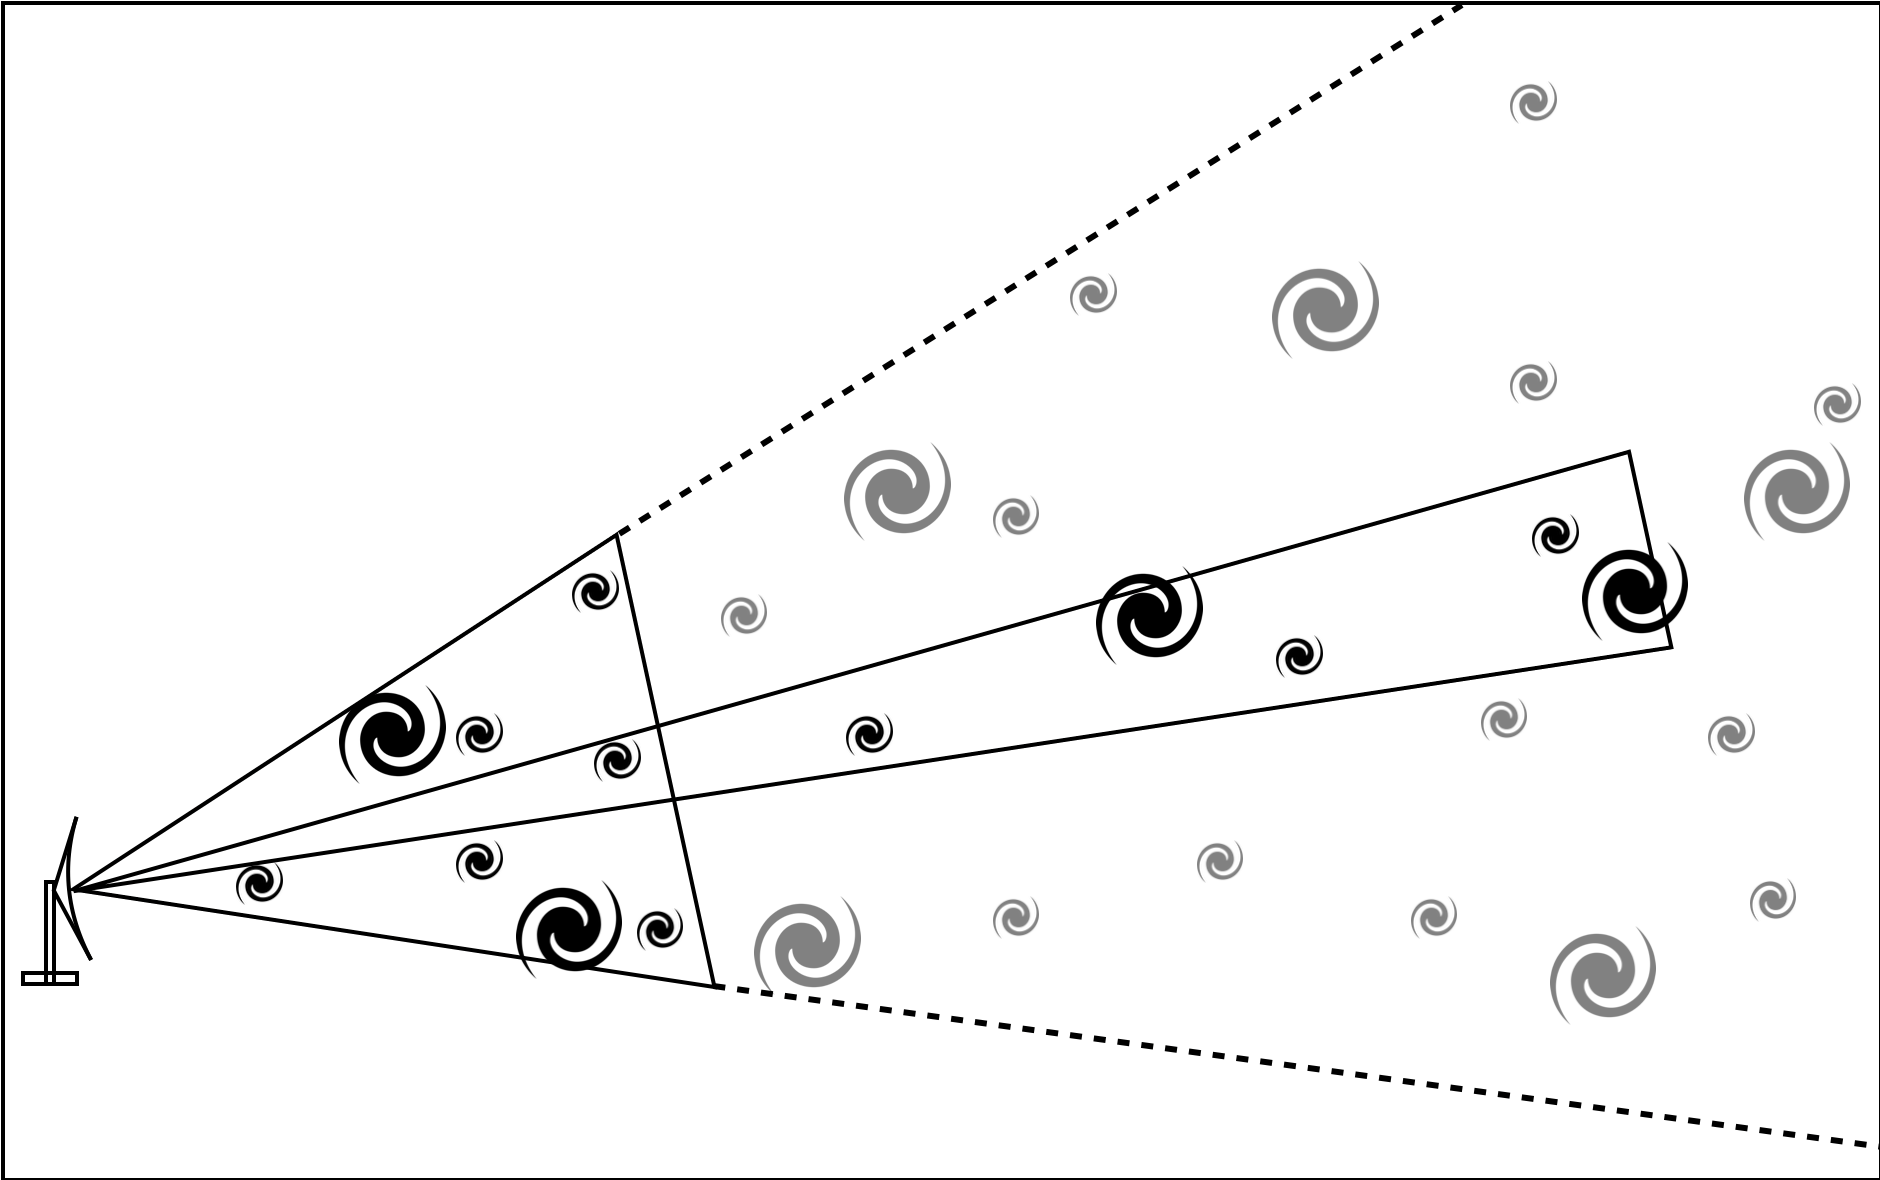
\includegraphics[width = \linewidth]{Figures/Chapter1/W_v_D_Toon.png}
    \caption{A simplified visualisation of how a trade-off is made between width and depth in surveys. Given two observation areas, the telescope is able to pick up galaxies to a much greater depth in narrow observation. By spending more time on one area of the sky the telescope can pick up more photons and therefore observe to a greater depth.}
    \label{fig:WvD}
\end{figure}

In addition, larger galaxies are significantly brighter (the example in Figure \ref{fig:Vmax} uses two galaxy size examples). The smaller galaxies can be observed to the solid line and the larger galaxies to the dashed line. The telescope observes 6 small galaxies and 5 large galaxies, however as the larger galaxies are brighter and can be seen to a greater depth. Corrections are therefore made to the number density of galaxies based on the depth that the galaxy can be observed to. In the 2D example from Figure \ref{fig:Vmax} the small galaxies can be seen in an area given by the solid area which we can call 1 unit$^2$ the larger galaxies can be seen in an area given by the dashed area that is 4 unit$^2$. In this example, the smaller galaxies have a number density of 6 galaxies p.u. area, the larger galaxies 1.25 galaxies p.u. area.

\begin{figure}[h]
    \centering
    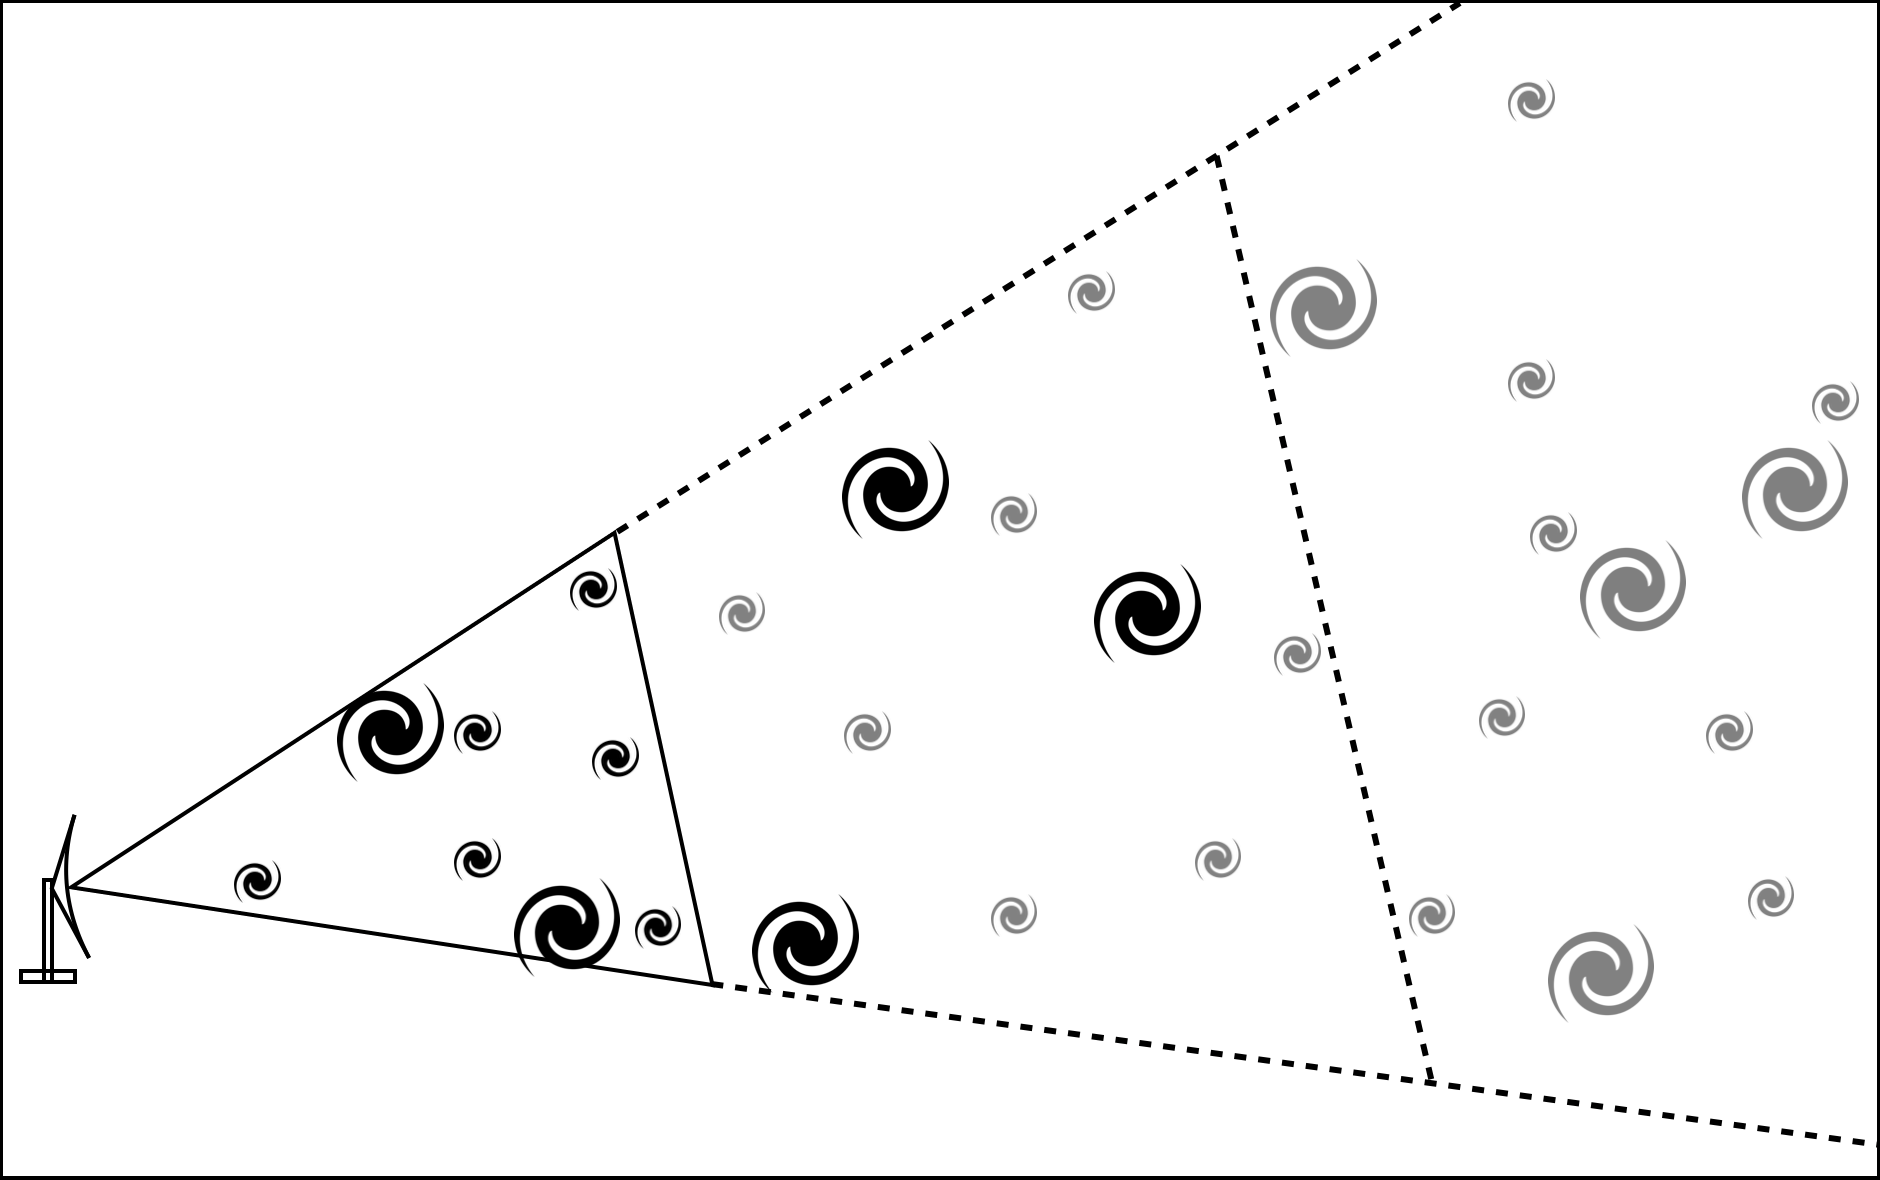
\includegraphics[width = \linewidth]{Figures/Chapter1/Vmax_Toon.png}
    \caption{A simplified visualisation of how the brightness of galaxies effects the observation depth. The smaller dimmer galaxies can be seen in the solid cone, larger and brighter galaxies can be seen up to the limits of the dashed cone.}
    \label{fig:Vmax}
\end{figure}

For each galaxy luminosity observed in a survey, a correction must be made by the total depth it could have been observed to and the associated volume. In this way, the volumetric density correction can be calculated for each galaxy in a given survey.

\subsubsection{Sloan Digital Sky Survey (SDSS)}

The Sloan Digital Sky Survey (SDSS) is arguably the premier wide survey for galaxies. SDSS started in 1998 with the mission to catalogue and map as much of the universe as possible. The latest release of the fourth phase is SDSS-DR19 \citep{Ahumada2019TheSpectra} now includes one-third of the night sky, it covers (u,g,r,i,z) wavelengths, has over 1.2 billion objects including over 200 million galaxies.

\subsubsection{CANDELS}
CANDELS (The Cosmic Assembly Near-infrared Deep Extragalactic Legacy Survey) observed galaxies in the redshift range z = 8 to 1.5. CANDELS uses three Hubble Space Telescope (HST) cameras to capture emission from mid-UV to near-IR for 250,000 galaxies. The primary goals of this survey of interest to this thesis is the observation of the peak of star formation and AGN activity at $z \simeq 2$ \cite{Grogin2011Candels:Survey}.

\subsubsection{COSMOS}

COSMOS: The Cosmic Evolution Survey is a 2 square degree survey covering many wavelengths using a combination of observation from many space-based and ground-based telescopes (Space: Hubble, Spitzer, GALEX, XMM, Chandra, Herschel, NuStar) (Ground: Keck, Subaru, VLA, ESO-VLT, UKIRT, NOAO, Badde and Blanco, CFHT). Combining the data allows COSMOS to create a rich view of the observed objects across a huge range of wavelengths. COSMOS was designed to observe galaxy evolution across cosmic time and understand the environmental effects of galaxies growing in groups and clusters \citep{HomeCOSMOS}.

\subsubsection{3D-HST}

Using 248 orbits and 124 pointings the 3D-HST is a highly complementary survey observing 625 arcminutes of previously observed extra-galactic fields \citep{Brammer20123D-HST:Telescope}. 3D-HST provides spectroscopic redshifts for over 10,000 galaxies in the range $1 < z < 3.5$. The survey provides 22 bands of rest-frame colours used for the redshift catalogues, the UV-IR star formation rates and, stellar masses. The primary science goal is to investigate the evolution of galaxies at high redshifts and in combination with CANDELS be the primary spectroscopic data set until the launch of JWST.

\subsection{Future Surveys}

Due to the pace of technological advancements and the difficult and expensive nature of building (and launching in the case of space-based missions) telescopes, our current survey telescopes are far behind what is theoretically possible. In this subsection two of the next generation survey telescopes are described. Both are space-based missions being launched into orbit at the second Lagrange\footnote{The Lagrange points are 5 distinct points in a gravitational two-body system at which an object can remain at rest relative to the two major bodies. In these points, the forces of gravitational acceleration, centripetal acceleration and for some points the Coriolis effect are all in balance.} point 4 times the distance between the moon and the earth. The second Lagrange point is unique in its position as it sits behind the earth and is therefore permanently in the earth's shadow. This positioning is ideal for satellites as it is also within the earth's magnetotail and therefore experiences lower solar wind irradiation. The drawback of this point is that from here any faults that are present at launch or develop during the operation of the missions will be permanent as it is not possible to retrieve and/or fix objects sent to these points.

\subsubsection{JWST \cite{JamesNASA}}

The James Webb Space Telescope is a cold infrared telescope with a planned launch in 2021\footnote{Correct at time of writing, JWST has some notoriety for pushing this date back}. Using multi-object near-infrared spectroscopy JWST will be able to take spectra for ~100 galaxies simultaneously. Galaxies will be observed in the redshift range $1 < z < 7$ covering the peak of cosmic star formation and much of their early formation. JWST is an infrared survey is particularly suited to probe the star formation of galaxies, the buildup of the Hubble sequence, the formation of metals, or the effects of starbursts \cite{Windhorst2009JWST2009}.  


\subsubsection{EUCLID}

The EUCLID satellite will carry two instruments VIS \& NISP. Between them they will cover from 500nm to 2000nm wavelengths down to the 24th magnitude, providing images of galaxies up to redshift $z = 2$. Euclid will survey 15,000 deg$^2$ of the sky and then perform a deep survey covering 40 deg$^2$ to 2 magnitudes deeper. The primary mission goals of Euclid are to address open questions on dark matter, dark energy, cosmic expansion and the formation of large scale structures \cite{Amendola2018CosmologySatellite}. To address these questions galaxies will be used as tracers of dark matter that providing tests of cosmological models. To achieve this goal the EUCLID pipeline will contain advanced galaxy cluster detection algorithms \cite{Adam2019EuclidSelection}.


\section{$\steel$}

There are several outstanding issues in galactic astrophysics that the models and techniques described in this section are not able to comprehensively address. In this thesis, we will describe the development of \steel as a tool to be able to directly address these issues by introducing a new modelling paradigm. 


Firstly, we address the reproduction and evolution of the full stellar mass function history, including satellite and central galaxies over a wide range of masses. This has proven problematic for semi-analytic models \cite{Asquith2018CosmicModels} and is essential to understand how galaxies have grown over cosmic time.
The importance of the full SMF reproduction is highlighted in Chapter \ref{Chapter:Method} where we show how \steel as an empirical model reproduces this by design. The generation of full satellite galaxy distributions is shown in Chapter \ref{Chapter:GalDist} and compared to the distributions of satellites locally and at high redshift. 

Secondly, in-situ (internal mass growth) vs ex-situ (mass growth from cannibalisation of other galaxies) invites several open questions: The total amount from each source, the characteristic mass at which galaxies switch from one mode to the other, e.t.c.  \cite[e.g.]{Cattaneo2011HowMass, Moster2018Emerge10, Behroozi2019UniverseMachine:010, Bernardi2011Curvature1011M, Shankar2015}. We use the empirically generated/constrained environments from Chapter \ref{Chapter:GalDist} to add constraints to these questions in Chapter \ref{Chapter:GalGrowth}.

Additionally, the selection of galaxy pair fractions and their evolution with redshift is in contention \citet{Man2016RESOLVING03, Mundy2017A3.5}. It is unclear if the pair fraction increases or decreases with redshift, which has implications for our ability to observationally estimate the galaxy merger rate. In Chapter \ref{Chapter:GalPairs} we show a systematic analysis of how the choice of stellar-mass estimation propagates into observed pair fractions.

Finally, the rate and significance of galaxy-galaxy mergers as predicted by \LCDM hierarchical assembly is a source of some debate \cite[e.g.][]{Hopkins2010MERGERSMATTER,Hopkins2009HOWMERGERS,Hopkins2010MergersFunctions,Fensch2017High-redshiftFormation,Martin2017TheTime}. A core prediction of mergers is that they drive the morphological change seen in galaxies between high and low redshift \cite[e.g.][]{Bournaud2011HydrodynamicsSpheroids,Bournaud2011StarMergers,Hilz2013}. To conclude \ref{Chapter:GalPairs} we use the statistical merger rate from obtained from \steel, alongside a statistical representation of several morphological change models that are driven by mergers. The results of these models are then compared to the morphological fractions in the local universe.

\section{Original Sources}

A large fraction of this thesis is a restructuring of three papers published during PhD studies by PJG. The papers are:
\begin{itemize}
    \item \textit{`A Statistical Semi-Empirical Model: Satellite galaxies in Groups and Clusters'}  \citet{Grylls2019AClusters}, hereafter \Paper{1}
    \item \textit{`Predicting fully self-consistent satellite richness, galaxy growth and starformation rates from the STastical sEmi-Empirical modeL \textsc{steel}.'} \citet{Grylls2020PredictingSTEEL}, hereafter \Paper{2}
    \item \textit{`The significant effects of stellar mass estimation on galaxy pair fractions.'} \citet{Grylls2020TheFractions}, hereafter \Paper{3}
\end{itemize}

Each chapter, including the introduction and conclusion, may contain work from all three sources however the major sources for each are as follows: Chapter \ref{Chapter:Method} reports primarily from \Paper{1} where the method was originally published, updates to the method from \Paper{2} \& \Paper{3} are also included. Chapter \ref{Chapter:GalDist} restructures the discussion of galaxy distributions from \Paper{1} \& \Paper{2}. Chapter \ref{Chapter:GalGrowth} presents the critical finding published in \Paper{2} and contextualises the main result in greater detail. Finally, Chapter \ref{Chapter:GalPairs} details the results from \Paper{3} and a work in preparation by SP for which PJG has acted as a supervisor in conjunction with FS. Where possible text and figures are reproduced in original form, however substantial reordering, alongside edits and additions have been selectively made to show how the work produced over PJG's candidature relate to one another and the wider field as well as to improve the `narrative'. The papers are produced in full in Appendix \ref{Appx:Papers}.
